\documentclass[12pt]{pylatex}
\usepackage{examples}
\usepackage{caption}
\usepackage{graphicx}

\makeatletter
\def\cm#1{\strip@pt\dimexpr #1*65536/\number\dimexpr1cm}
\def\inches#1{\strip@pt\dimexpr #1*65536/\number\dimexpr1in}

\begin{document}

\section*{Passing LaTeX data to Python}

There are occassions where the active Python code may require information from the LaTeX source. Since Python has no direct access to LaTeX some other means must be provided to build this bridge. The idea presented here follows a standard LaTeX pattern -- run LaTeX twice, once before Python, leaving breadcrumbs for Python to pickup during its run, then a final LaTeX run to complete the job.

The example shown here is a simple proof of concept. It shows how the dimensions of plot can be specified in the LaTeX source and then accessed later by Python.

To compile this example, use

\begin{lstlisting}
   pdflatex      example-09
   pylatex.sh -i example-09
\end{lstlisting}

The idea is to use LaTeX to create a Python dictionary saved as a {\tt\small .json} file. The dictionary will contain just two entries, one for the height and one for the width of the plot. Here are the relevant lines of LaTeX.

\vspace{10pt}

\begin{latex}
   \newdimen\mywidth\mywidth=17cm       % target width
   \newdimen\myheight\myheight=13.5cm   % target height

   \newwrite\breadcrumbs
   \immediate\openout\breadcrumbs=\jobname.json                % create Json file
   \immediate\write\breadcrumbs{\writebgroup}                  % {
   \immediate\write\breadcrumbs{"height":\inches{\myheight},}  %    "height":5.31496,
   \immediate\write\breadcrumbs{"width":\inches{\mywidth}}     %    "width":6.69292
   \immediate\write\breadcrumbs{\writeegroup}                  % }
   \immediate\closeout\breadcrumbs                             % close the file
\end{latex}

% https://tex.stackexchange.com/questions/47452/writing-and-to-a-file-with-latex
% macros to write { and }
\begingroup
\catcode`<=1 \catcode`>=2 \catcode`{=12 \catcode`}=12
\gdef\writebgroup<{> \gdef\writeegroup<}>
\endgroup
% or:
% \edef\writebgroup{\iftrue\string{\else}\fi}
% \edef\writeegroup{\iffalse{\else\string}\fi}

% set the width and height of the figure
\newdimen\mywidth\mywidth=17cm
\newdimen\myheight\myheight=13.5cm

% save width and height in a Python-Json dictionary
\newwrite\breadcrumbs
\immediate\openout\breadcrumbs=\jobname.json
\immediate\write\breadcrumbs{\writebgroup}
\immediate\write\breadcrumbs{"height":\inches{\myheight},}
\immediate\write\breadcrumbs{"width":\inches{\mywidth}}
\immediate\write\breadcrumbs{\writeegroup}
\immediate\closeout\breadcrumbs

The target dimensions are: (width, height) = (\cm{\mywidth} cm, \cm{\myheight} cm).

\lstset{numbers=left}

\vspace{5pt}

The following Python code does the job of reading the dictionary and setting the values of
{\tt\small height} and {\tt\small width}.

\vspace{5pt}

\begin{python}
   import io, os, json

   # read the dictionary
   try:
      with io.open(os.getcwd() + '/' + 'example-09.json') as inp_file:
         inp = json.load(inp_file)
   except:
      inp = { "width":"6.4",
              "height":"4.8" }

   # set figure dimensions in inches (yikes)
   width  = inp['width']
   height = inp['height']

\end{python}

\vspace{5pt}

This Python code does the job of plotting the Bessel functions (it is based on the code from example-04).

\vspace{5pt}

\begin{python}
   # plot the Bessel functions
   import numpy as np
   import scipy.special as sp
   import matplotlib.pyplot as plt

   plt.matplotlib.rc('text', usetex = True)
   plt.matplotlib.rc('grid', linestyle = 'dotted')
   plt.matplotlib.rc('figure', figsize = (width,height))

   x = np.linspace(0, 15, 500)

   for v in range(0, 6):
       plt.plot(x, sp.jv(v, x))

   plt.xlim((0, 15))
   plt.ylim((-0.5, 1.1))
   plt.legend(('${J}_0(x)$', '${J}_1(x)$', '${J}_2(x)$',
               '${J}_3(x)$', '${J}_4(x)$', '${J}_5(x)$'), loc = 0)
   plt.xlabel('$x$')
   plt.ylabel('${J}_n(x)$')
   plt.grid(True)

   plt.tight_layout(pad=0.5)

   plt.savefig('example-09-fig.pdf')

   width_cm  = round (width  * 2.54, 2)   # py (width,width_cm)
   height_cm = round (height * 2.54, 2)   # py (height,height_cm)
\end{python}

The following figure should have dimensions: (width, height) = (\py{width} cm, \py{height} cm).

\vspace{10pt}

\begin{minipage}{\textwidth}
   \centering
   \IfFileExists{example-09-fig.pdf}%
   {\fbox{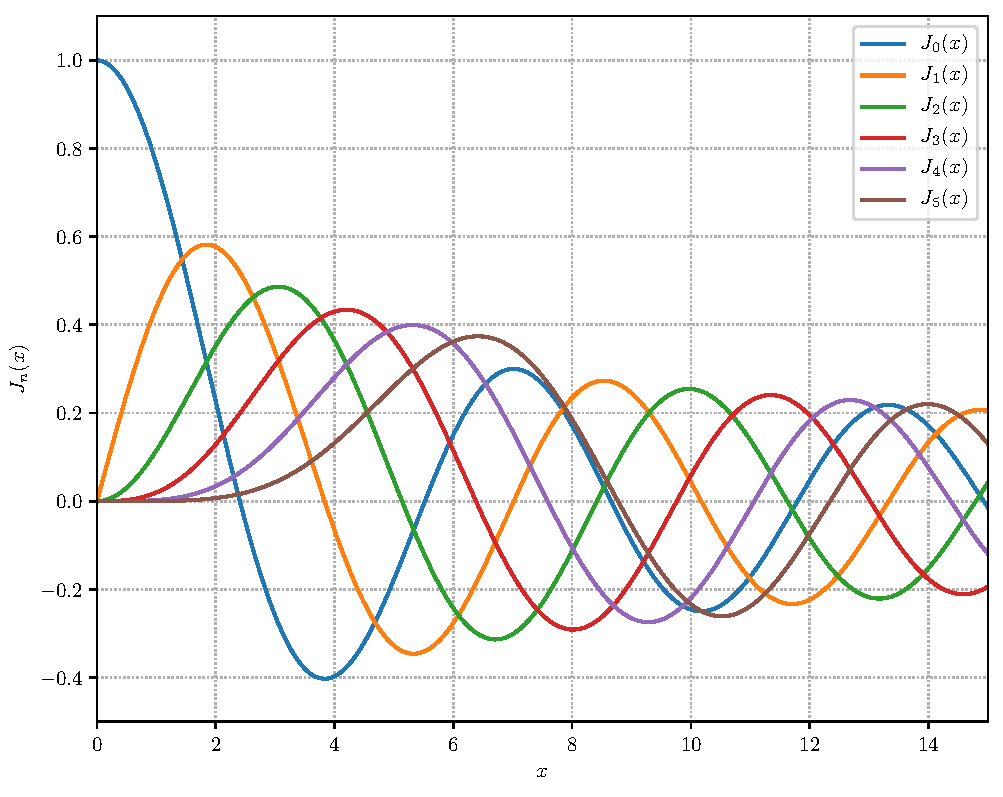
\includegraphics
      {example-09-fig.pdf}}}{Failed to create pdf plot.}
   \captionof{figure}{The first six Bessel functions.}
\end{minipage}

\end{document}
